%\documentclass[sigconf]{acmart}
%\documentclass[sigconf,10pt,anonymous]{acmart}
\documentclass[sigconf,10pt]{acmart}

\usepackage{balance} % For balanced columns on the last page
\usepackage[english]{babel}
\usepackage{blindtext}
\usepackage{subcaption}
\usepackage{xspace}

% Copyright
\renewcommand\footnotetextcopyrightpermission[1]{} % removes footnote with conference info
\setcopyright{none}
%\setcopyright{acmcopyright}
%\setcopyright{acmlicensed}
%\setcopyright{rightsretained}
%\setcopyright{usgov}
%\setcopyright{usgovmixed}
%\setcopyright{cagov}
%\setcopyright{cagovmixed}

\settopmatter{printacmref=true, printccs=true, printfolios=false} %folios not allowed for Mobi 20'

%\copyrightyear{2020}
%\acmYear{2020}
%\setcopyright{acmcopyright}
\acmConference[CE7490]{Distributed Systems}{Semester 1}{Nanyang Technological University, Singapore}

\begin{document}
\title{RAID-6 atop S3}

\author{Ismail Lotfi and Amalinda Gamage}

 \affiliation{
    \department {School of Computer Science and Engineering}
   \institution{Nanyang Technological University}
   \city{Singpore}
 }
 \email{{ismail003,jath0001}@e.ntu.edu.sg}

\begin{abstract}
Inexpensive, reliable storage is increasingly required for both businesses and the homes.
As disk capacities increase and multiple drives are combined in one system, the probability of multiple disk failures increases.
An idea originally refereed as \textit{Redundant Array of Inexpensive Disks}  (RAID) and now refereed as \textit{Redundant Array of Independent Disks} RAID proposes a range of RAID versions to solve this problem.
This work focuses on RAID-6.
RAID-6 is an improvement to the functionality of RAID-5 by an additional block of parity and tolerates up to two arbitrary concurrent disk failures.
The key contribution of our work is the implementation and evaluation of a basic RAID-6 system atop multiple geo-distributed S3 storage buckets.
We briefly state below several additional advanced features this RAID-6 implementation offers.
First our implementation incorporates an unlimited files of arbitrary names and sizes.
The unlimited nature in the number of files is the result of exploiting S3 object storage buckets as the main storage medium.
Second, it supports a range of user intended RAID-6 disk configurations such as numbers of data, parity disks and file chuck sizes.
Lastly, it also handles automatic detection of S3 object based storage disk failures as well their recovery.
Our implementation is available at: \url{https://github.com/Amalinda/RAID6}.
\end{abstract}

\begin{CCSXML}
<ccs2012>
   <concept>
       <concept_id>10003033.10003058.10003065</concept_id>
       <concept_desc>Networks~Wireless access points, base stations and infrastructure</concept_desc>
       <concept_significance>500</concept_significance>
       </concept>
</ccs2012>
\end{CCSXML}
\ccsdesc[500]{Storage~Redundancy, S3 and RAID-6}

\keywords{Geo-distributed Reliable Storage}

\maketitle

\section{INTRODUCTION}
\label{sec:intro}

The  most  common  solution  for  the  provision  of  reliable data  storage  is  Redundant Arrays of Independent Disks (RAID) that enables multiple storage elements to be combined to offer a combination of better performance and tolerance to failure.
As RAID systems help achieve a user desired balance between cost, reliability and capacity, they have enjoyed ubiquitous widespread popularity as storage mechanism~\cite{raid_survey}. Several RAID architectures have been proposed. This paper focuses on RAID-6 systems.

While RAID-5 uses only one parity block, RAID-6 extends RAID-5 by adding another parity strip. This allows for two disk failures within the RAID set before any data is lost. The larger the drive capacities and the larger the array size, the more important it becomes to choose RAID 6 instead of RAID-5~\cite{raid6_stop_2019}. Moreover, in current data centers where there are thousands of hard disks, more concurrent disk failures are more frequent, which motivate the need to use systems that tolerate more failures such as RAID-6~\cite{Failure_Trends_2007}.

In this work, we go through a detailed explanation of RAID-6 core design followed by an implementation of this system on top of S3 buckets. Due to the competitive prices on cloud storage, many companies and individuals are using S3 buckets to store their data in different regions~\cite{cloud_2020}. However, some users might want more reliability for their data instead of relaying on a third party implementation. An interesting approach to so is by implementing the RAID-6 system on top of the S3 buckets. We present our detailed analysis of the proposed model and present other possible directions and improvement. 



\begin{figure*}
    \centering
    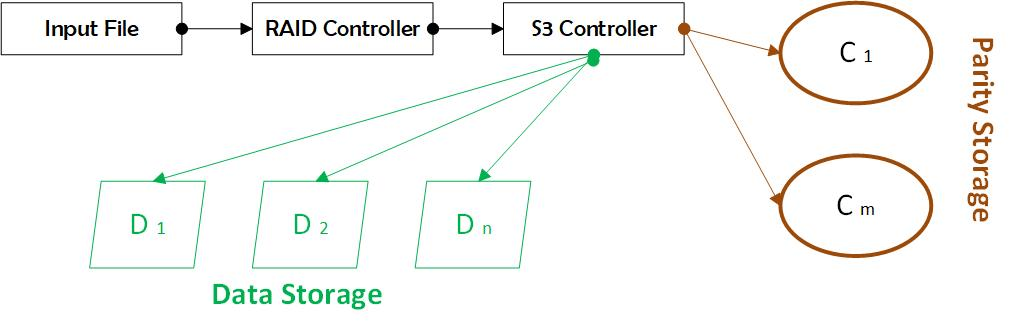
\includegraphics[width=\textwidth]{figures/over_0.jpg}
    \caption {Overview of the S3 based RAID-6 storage architecture}
    \label{fig:overview}
\end{figure*}




The remainder of this paper is organized as follows. In
Section 2, we present our system architecture. Section
3 describes the implementation process. Section 4 shows the experiments conducted and section 5 highlight the lessons leaned and some limitations.





\section{PRIMER ON S3 AND RAID-6}
\label{sec:primer}

In this section we provide the reader a basic understanding of the mathematics behind the operation of RAID-6 as well as S3 object storage.

\subsection{Object Storage for RAID}
Typically, the equivalent of a single unit of S3 storage compared to a typical storage such as a hard disk is called a "bucket"\footnote{In what follows, we use the terms object storage and S3 interchangeably.
}. 
Object storage offers several advantages compared to traditional hard disk based file storage systems.
Almost all vendors offer salable object storage by means of \textit{elastic S3 buckets}.
This implies that maximum storage size of a RAID array made of S3 buckets need not be decided a priory.
As such, the total size of a RAID system made of S3 buckets could easily scale with the total size of the files stored in all S3 buckets, i.e, if the total size of files decreases, the total size of the RAID system decreases thereby, decreasing the monthly cost of the RAID system vice versa.
In addition, vendors also offer users the facility to instantiate S3 buckets across many regions of the world.
This significantly enhances the reliability of the data stored under RAID systems that utilize geo-distributed S3 buckets.
By extension, since all S3 buckets are managed by vendors, the S3 based RAID are not burdened with typical maintenance problems that arise from typical physical disk based RAID systems.

However, object storage is not with no disadvantages.
Object storage systems differ significantly from typical file storage systems in that they cannot be accessed by standard *nix file operation calls.
As such, the only method of storing, retrieving and modifying data within an S3 bucket requires network access.
Following that, all file operations are capped and reliant on network speed. Luckily, with its growing influence on individual consumers and large economies alike, the internet has become an increasingly vital part of our day-to-day lives and most of the people around the world are able to connect with high speed~\cite{statistica_2020, speedTest_2020}.

\subsection{RAID-6 Arithmetic}
\label{raid_arithmetic}
In RAID-6, failure of a disk is modeled as an erasure, i.e., the failure of a storage device denotes a shutdown or no data to/from the device \footnote{Note that this is different to reading incorrect bits off a storage device. RAID-6 does not innately handle such failures.}.
The RAID-6 arithmetic involves three major aspects.
First the Vandermonde matrix is utilized to calculate and to maintain the checksum words on parity disks~\cite{raid6_2011}.
Gaussian Elimination method is used to recover when an error is detected.
A Galois field is used to perform arithmetic.
We describe each of these steps in detail below. 
\\[1pt]

\noindent {\bf Computing and Maintaining Parity:}  The framework of a RAID-6 system is shown in Figure~\ref{fig:overview} . Assume that the RAID-6 system consists of $N$ data disks, $D_{1}, D_{2}.. D_{N}$ and $M$ parity disks $P_{1}, P_{2}.. P_{M}$ each holding only \textit{chuck size} of bytes.
The data of each parity disk is computed using data from the data disks.
The idea is that at any moment of time, a maximum of $M$ disk failure could simultaneously fail while still leaving the ability to reconstruct original data from the remaining disks.
The function to compute the content of parity of disk $i$ is $F_i$ and it takes as arguments all the data present in data disks as represented in Eq-\ref{eq:parity}.

\begin{equation}
\label{eq:parity}
P_i = F_i(D_1,D_2,...,D_N) = \sum_{j=1}^{N}d_j f_{i,j}
\end{equation}

Then all data chunks are aggregated to be a matrix $D$ where $D = [d_1, d_2,..,d_i]$ and all parity into a matrix $P$ where $P = [p_1, p_2,..,p_i]$.
Therefore, the state of the system can be defined as $P = FD$.
The computation of $P$ requires the generation of $F$, an $M \times N$ matrix called the Vandermonde matrix where $f_{i,j}=j^{i-1}$.
A verbose version of this computation is expressed in Eq-\ref{eq:parity1} and Eq-\ref{eq:parity2}.
It should be noted that this parity calculation should be carried out by performing the matrix multiplication over a Galois Field~\cite{matrix_1991}.

\begin{equation}
\label{eq:parity1}
P= \left[
\begin{matrix}
f_{1,1}      & f_{1,2}      & \cdots & f_{1,N}      \\
f_{2,1}      & f_{2,2}      & \cdots & f_{2,N}      \\
\vdots & \vdots & \ddots & \vdots \\
f_{M,1}      & f_{M,2}      & \cdots & f_{M,N}      \\
\end{matrix}
\right]
\left[
\begin{matrix}

D_{1} \\
D_{1} \\
\vdots \\
D_{1} \\
\end{matrix}
\right]
\end{equation}

\begin{equation}
\label{eq:parity2}
P= \left[
\begin{matrix}
1      & 1      & \cdots & 1      \\
1      & 2      & \cdots & N      \\
\vdots & \vdots & \ddots & \vdots \\
1      & 2^{M-1}      & \cdots & N^{M-1}      \\
\end{matrix}
\right]
\left[
\begin{matrix}

D_{1} \\
D_{1} \\
\vdots \\
D_{1} \\
\end{matrix}
\right]
\end{equation}

\noindent {\bf Recovery of Disks:} In order to illustrate the recovery from disk failures, we define a matrix A and E such that $A = \left[\begin{matrix}I \\F \\\end{matrix}\right]$, and $E= \left[\begin{matrix}D \\P \\\end{matrix}\right]$ which aids in developing the relation $AD = E$.
Here, $I$ is a $N \times N$ identity matrix and matrix $F, D, P$ are described as before. 
As shown, each storage device in the system can be viewed as having a corresponding row in the matrix $A$.
When a failure is detected, it is reflected in this equation by deleting the corresponding content of the failed device from $A$ and from $E$ resulting $A'$ and $E'$.
This modifies the existing equation to $A'D = E'$.

Elaborately, should data disk $D_{i}$ and parity disk $P_{j}$ fails simultaneously, the the $i^{th}$ row of $I$ and $j^{th}$ row of $F$ should be deleted to generate the $A'$.
Afterwards, the $i^{th}$ row in $D$ and the $j^{th}$ row of $D$ should be deleted to generate the new $E'$~\cite{raid6_2011}, resulting in Eq-\ref{eq:gauss}

\begin{equation}
\label{eq:gauss}
D=A'^{-1}E'
\end{equation}

The desired matrix to be computed now is $D$.
To do so, $A'^{-1}$ is computed via the Gaussian Elimination method over a Galois Field followed by solving for $D$~\cite{matrix_1991}.






      

\section{System Implementation}
\label{sec:implementation}
In this section we describe the implementation of the RAID-6.

\subsection{Configuration}
Before the system is instantiated, a user is expected to configure the system.
The configuration parameters are described in table-\ref{table:config}.

\begin{table}[H]
\begin{tabular}{|l|l|}
\hline
\textbf{property} & \textbf{description}              \\ \hline
endpoint          & describes the location of buckets \\ \hline
access\_key       & required for authentication       \\ \hline
secret\_key       & required for authentication       \\ \hline
\ data disks      & number of data disks              \\ \hline
\ parity disks    & number of parity disks            \\ \hline
chuck size        & size in bytes for use as a chuck  \\ \hline
\end{tabular}
\caption{Mandatory system configuration parameters}
\label{table:config}
\end{table}

The parameter \textit{endpoint} is a URI that defines physical location of the S3 bucket.
All vendors offer S3 buckets physically located across various geographical regions.
If a user desires, it is possible to define $(N + M)$ different URIs corresponding to different geographical regions for higher storage reliability.

\subsection{Extending S3 as storage for RAID-6}

The RAID-6 functionality was first implemented and tested within a local machine.
It was then extended to utilize S3 API for all file operations as well as to perform fault detection and disk creation instead of *nix system calls.
This required creation of our own python-based functions to execute the expected input/output file operations in S3 buckets.
In our system, we assume one storage disk as a single S3 bucket.
Therefore, an implementation with four data disks and two parity disks will consist six S3 buckets.
We follow the standard S3 API documentation available at \cite{wasabiDocs}.
We chose Wasabi \cite{wasabiS3} as they do not charge extra for network quota at the time of writing.
In order to validate the functionality of the RAID-6 system, we also need to mimic \textit{disk failures}.
A separate program is made available in the source which aids in deleting arbitrary S3 buckets.

During the initialization, \textit{S3 controller} creates the desired number of S3 buckets to be used as disks.
It is imperative to note that bucket names need to be unique across a region.
Hence, to avoid conflicts, a unique name may be pre or post append to each bucket's name.
However, in our implementation, this need not be done as bucket name $disk\_i$ where $i$ ranges from $1-10$ were first claimed by us.

\subsection{Data Distribution and File Management}

\noindent {\bf File Storing:}
A single stripe consists $N$ data chunks and $M$ parity chunks.
In our implementation we utilize six data disks and two parity disks with a chunk size of 16 bytes.
For each new file added, the RAID-6 controller produces one or more chunks per each storage disk depending on the size of input file.
Chunks belonging to the same file are aggregated as a single file and are awarded the object name identified by the input file name.
I.e., a single input file will always cause $(N + M)$ files created in all buckets identified by the exact filename.
This provides the additional advantage of even updating the file at a later stage without no loss of storage space due to changed file sizes.
This is because each time an object is updated with the same name within an S3 bucket, the former space allotted for the said object no longer used or need to be paid for.
Coincidentally, this makes multiple file management comparatively easier due to innate advantages of S3 object storage.

\noindent {\bf File Retrieval:} Provided no disk failures are detected, when a file needs to be retrieved, corresponding objects identified by the requested filename from all S3 disks are downloaded to a local storage by the RAID-6 controller followed by simple reconstruction.

\noindent {\bf Recovery:}
Prior to performing any I/O operations on the RAID-6 array, the RAID controller always checks for failures.
Upon detecting a failed disk(s), as long as the simultaneous failure is less than $M$ number of disks, the RAID controller follows the process described in Section-\ref{raid_arithmetic} to repair the disks.
Even if buckets (disks) are completely deleted from the vendor storage, our implementation will re-create the lost buckets and re-generate lost data.

More specifically, the RAID-6 controller obtains a list of files from a working bucket and iterates through each possible object to obtain a list of files.
It then proceeds to reconstruct the data in lost buckets and uploads back.
Our expose a function RAID.Rebuild() from our RAID controller which achieves the aforementioned recovery functions and could be called arbitrarily to check and recover from disk failures.








\section{Evaluation}
\label{sec:evaluation}

Here we perform two experiments to quantify the performance of the S3 RAID-6 system and draw several conclusions based on our results.

First we experimentally determine the time required to distribute a file in the S3-RAID-6 array.
We call this the file store duration.
We estimate file store duration for a range of file sizes and report our results in Fig.\ref{fig:S3R6Str}.

Next we run an experiment to estimate the recovery time of the system from failures.
Our experiment methods is as follows.
First, we store a file of known size in the S3-RAID6 array.
Second, we choose $M$ number of random disks and delete them.
Thirdly, we start the timer and estimate the recovery duration.
During the recovery process, data from all buckets (disks) are downloaded by the RAID controller. 
It then checks for missing disks, reconstructs the lost data and re-uploads the same.
The timer is stopped after a successful re-upload.
We repeat this process for a range of file sizes and report our results in Fig.\ref{fig:S3R6Rcv}.
As expected, our results suggest that the performance of our system is strongly correlated with network speed.

\begin{figure}[h!]
\centering
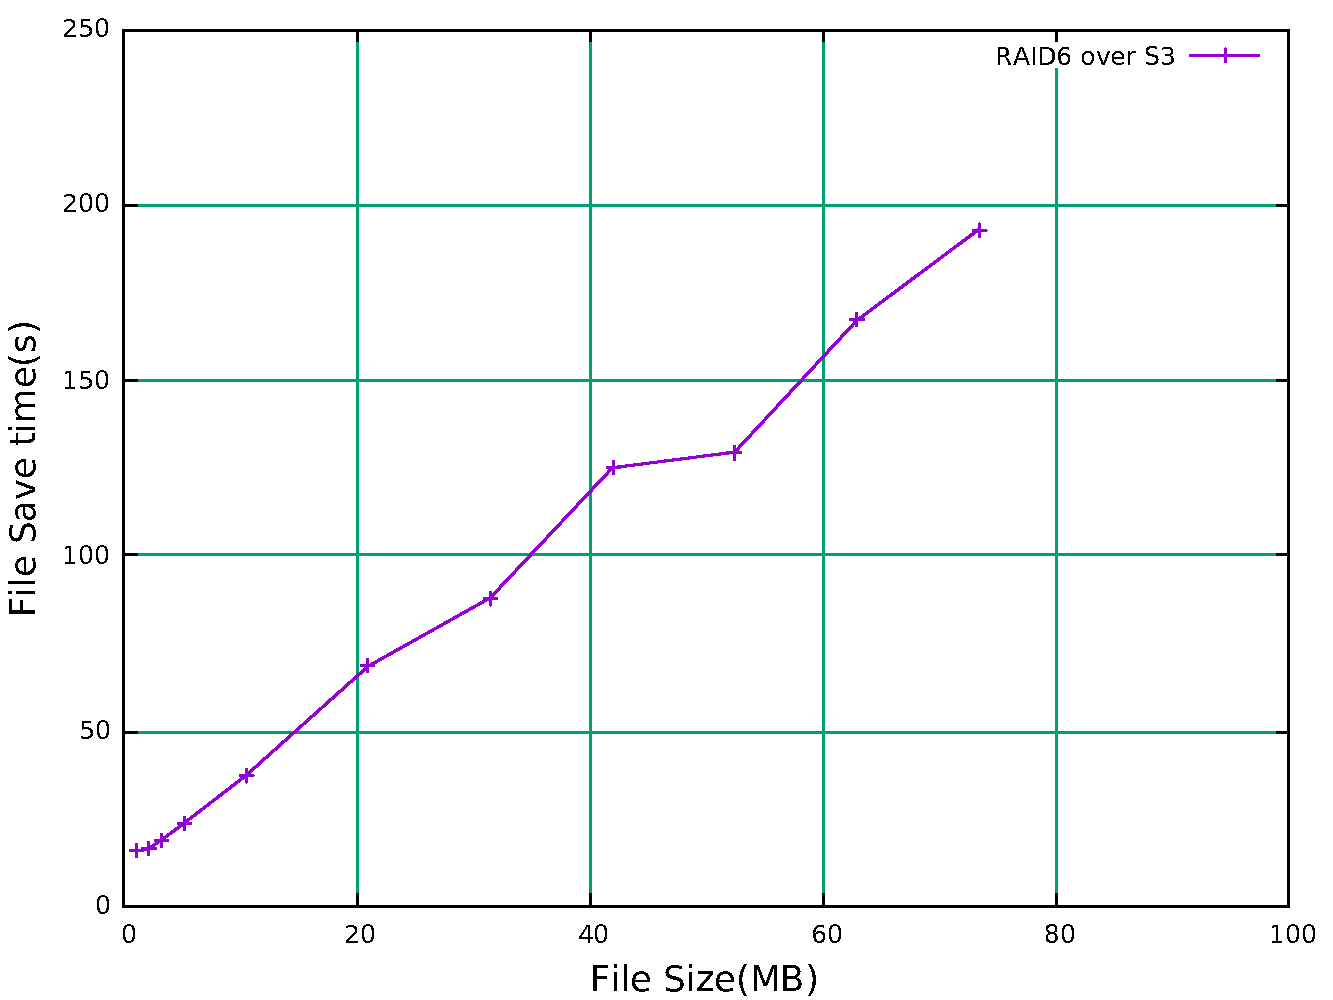
\includegraphics[width=\linewidth]{figures/S3RAIDStoreTime.pdf}
\caption{Time duration in seconds to store a file in S3 for varying file sizes.}
\label{fig:S3R6Str}
\end{figure}

\begin{figure}[h!]
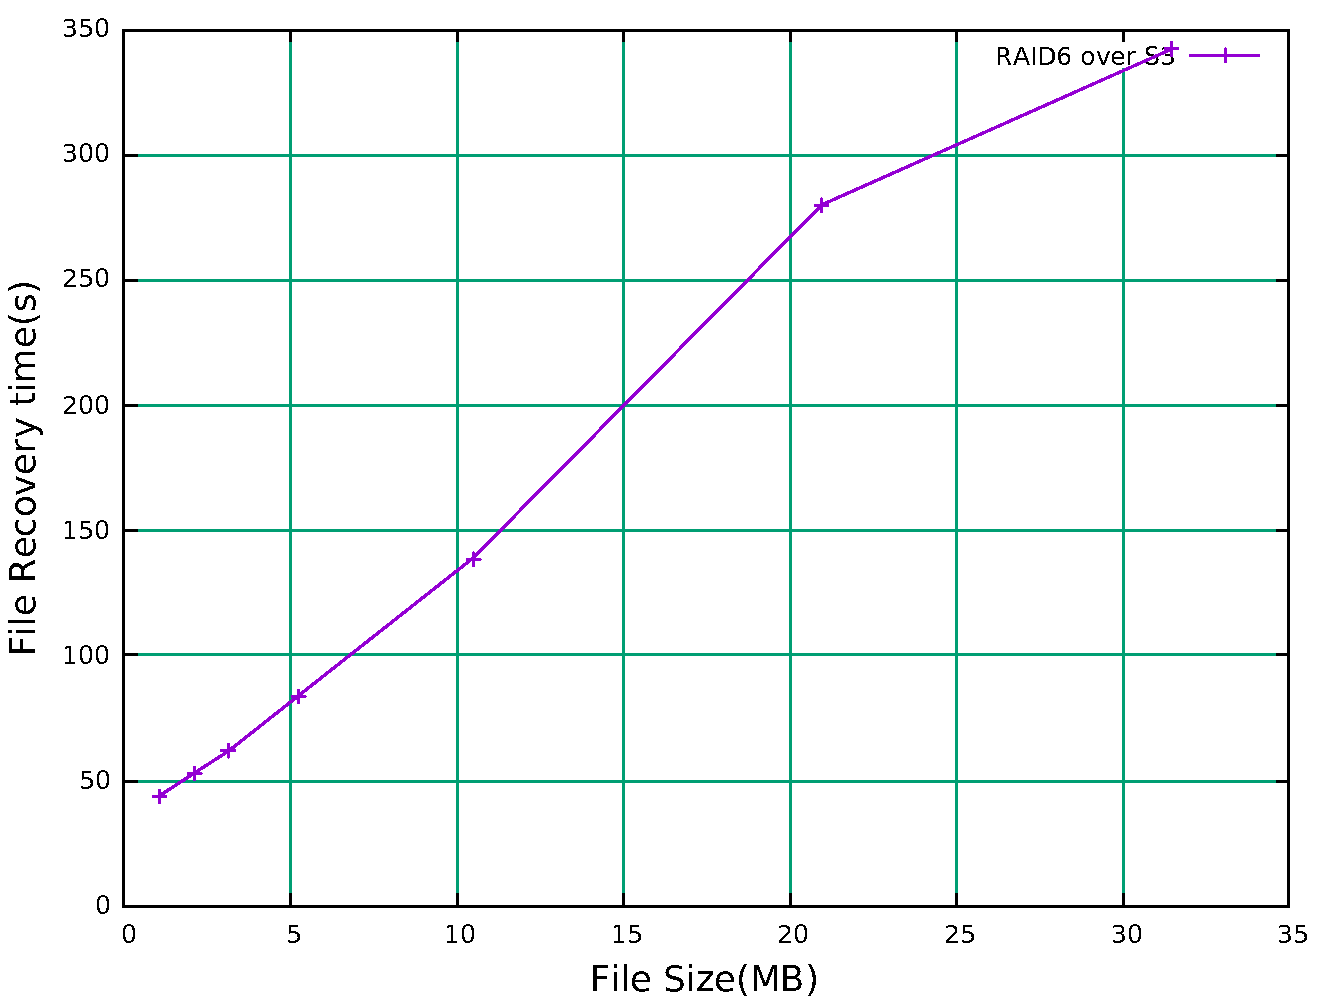
\includegraphics[width=\linewidth]{figures/S3RAIDRecoveryTime.pdf}
\centering
\caption{The Recovery time in seconds of $M=2$ deleted buckets(disks) for varying file sizes.}
\label{fig:S3R6Rcv}
\end{figure}

Afterwards, we quantity the effect of varying chunk size on file store and disk recover time.
To be thorough, we repeat the following experiment for 2 files of size 1MB and 5MB.
For each file we change the chunk size of the S3-RAID6 array varying from $8, 16, 32, 64, 128, 256$. For each file of 1MB and 5MB, we estimate the variation of file save time in Fig.\ref{fig:S3R6StrCHK1MB} and Fig.\ref{fig:S3R6StrCHK5MB}.
Afterwards, we then delete a single bucket from the S3-RAID6 array and compute the recovery time for each chunk.
We present this result in Fig.\ref{fig:S3R6RcvCHK1MB} and Fig.\ref{fig:S3R6RcvCHK5MB}. 
We observe that there is no strong effect of chunk size on file store and recovery time.
However, doubling the file size doubles file store time but increases file recovery time by a factor of three.
The minimal effect caused by chunk size highlights that the bottleneck for data storing and recovery is network throughput.
Furthermore, the raid controllers data/parity computation requires less time as opposed to reconstruction.
This is explained by the extra addition of upload time upon reconstruction as well as the reconstruction time which are similar in nature under the given file sizes and network throughput.

\begin{figure}[h]
\centering
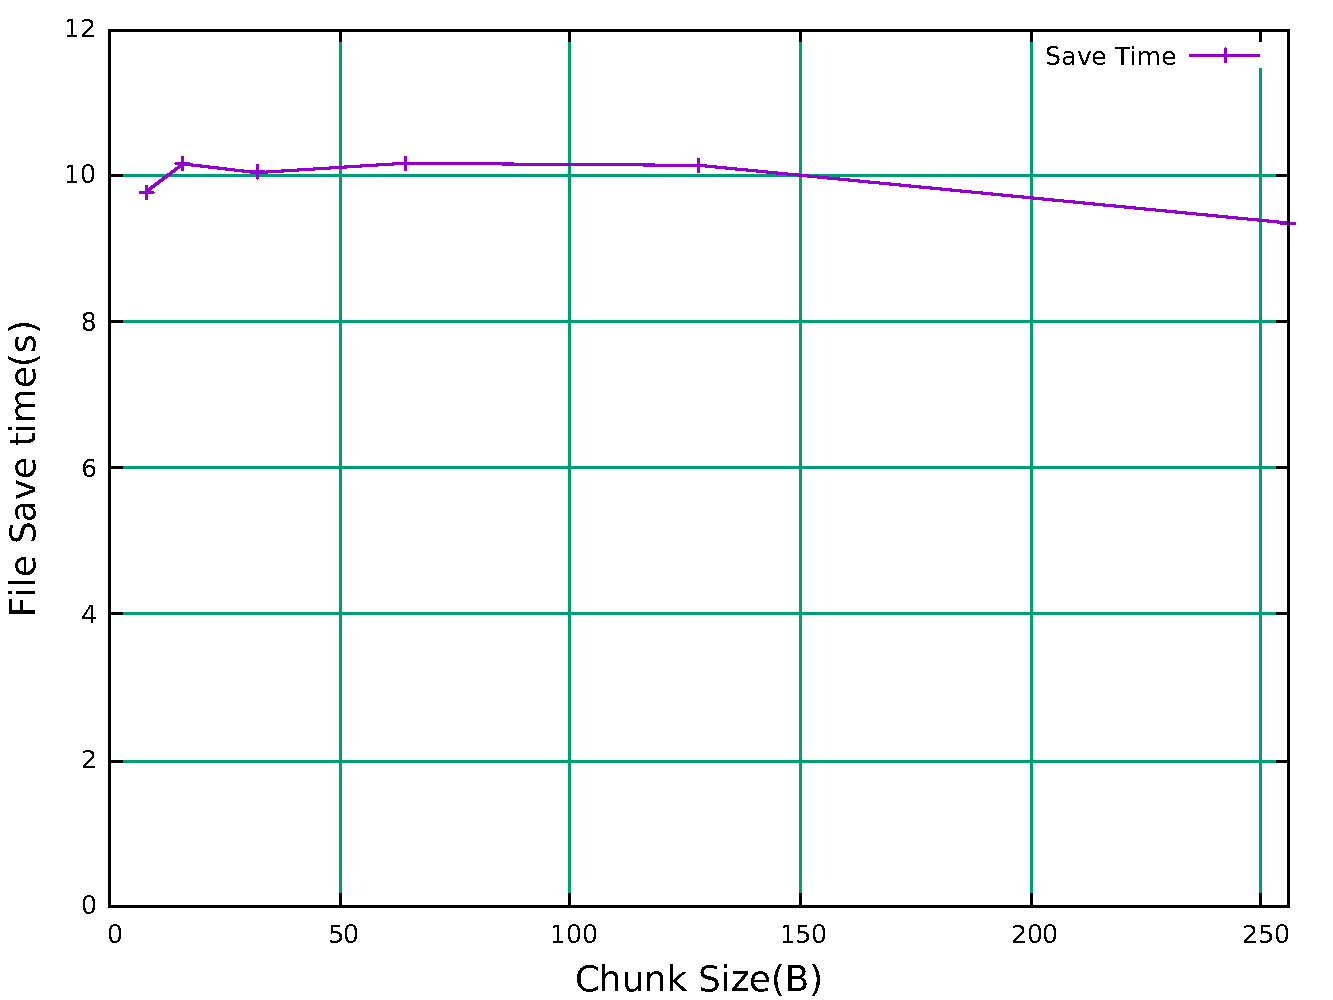
\includegraphics[width=\linewidth]{figures/RAIDStoreTimeChuckSize1Mb.pdf}
\caption{Time duration in seconds to store a file in S3 for varying Chunk sizes under a fixed file size of 1MB}
\label{fig:S3R6StrCHK1MB}
\end{figure}

\begin{figure}[h]
\centering
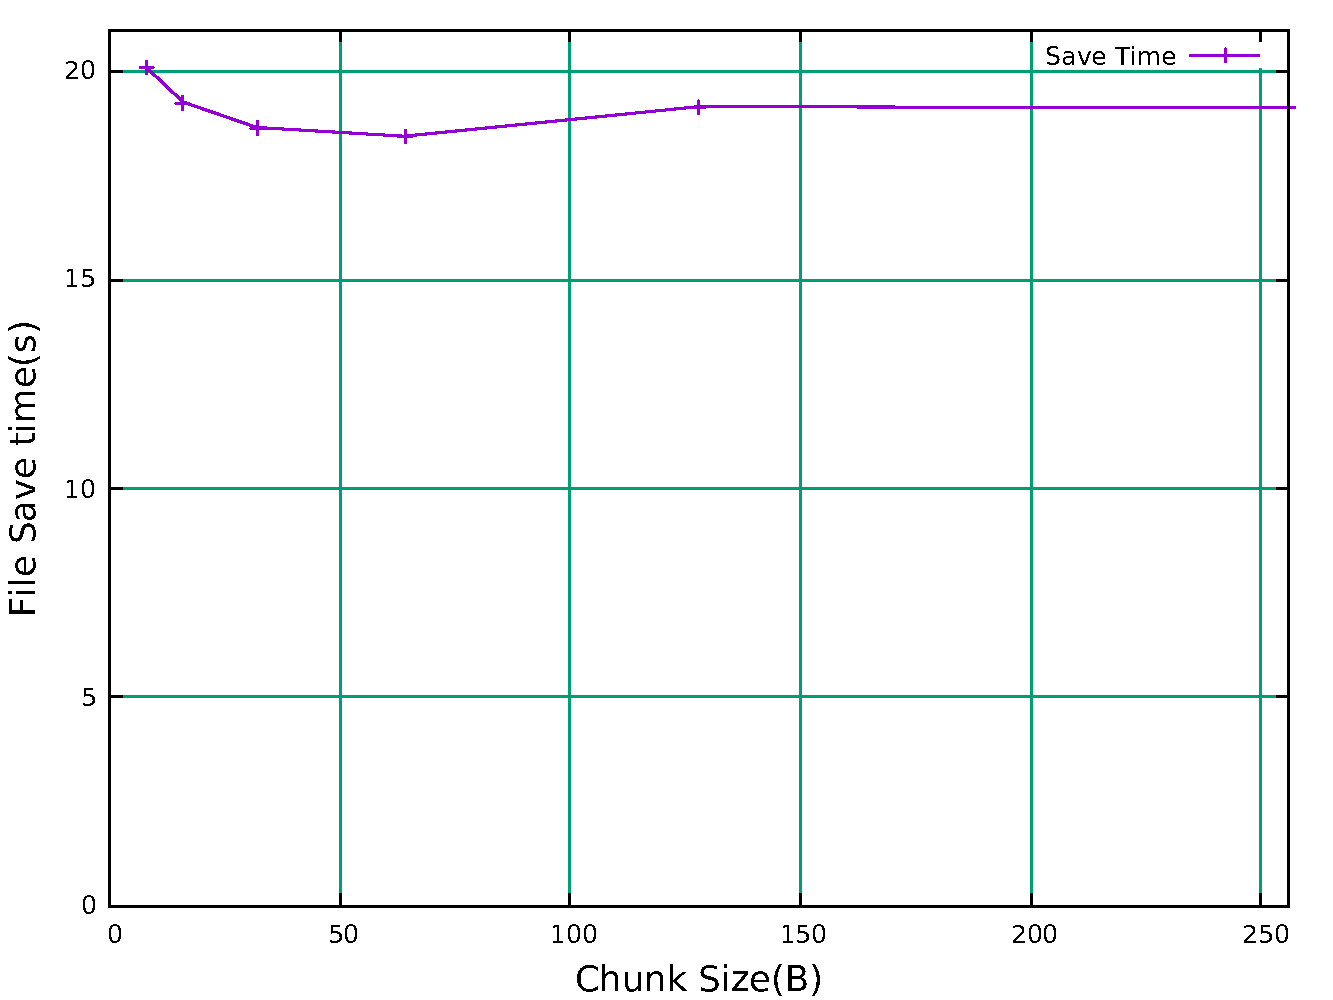
\includegraphics[width=\linewidth]{figures/RAIDStoreTimeChuckSize5Mb.pdf}
\caption{Time duration in seconds to store a file in S3 for varying Chunk sizes under a fixed file size of 5MB}
\label{fig:S3R6StrCHK5MB}
\end{figure}

\begin{figure}[h]
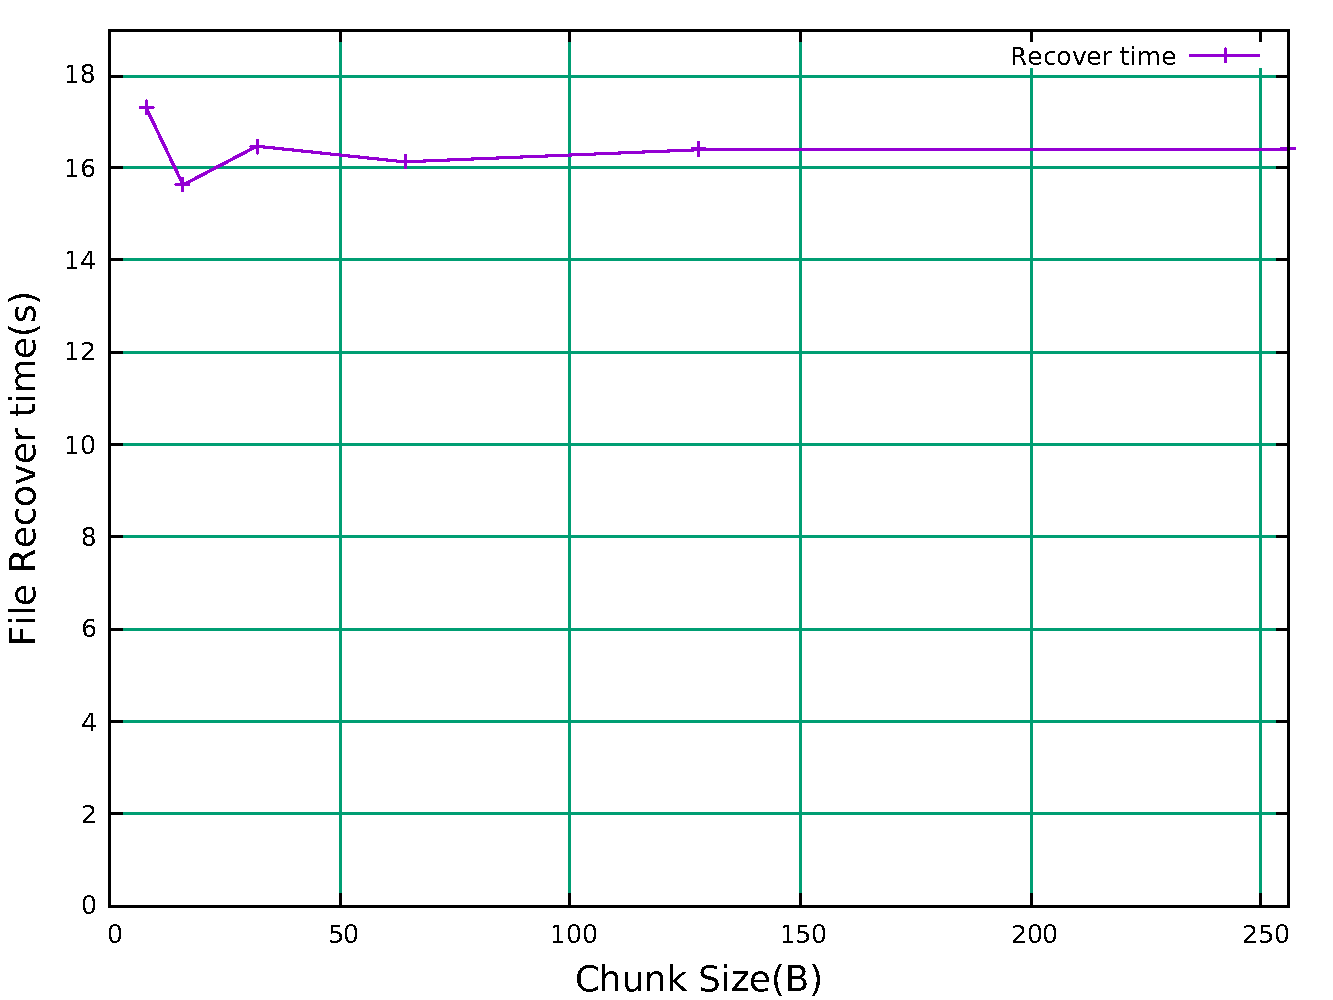
\includegraphics[width=\linewidth]{figures/RAIDRecoverTimeChuckSize1Mb.pdf}
\centering
\caption{Disk Recover time in seconds for varying Chunk sizes under a fixed file size of 1MB}
\label{fig:S3R6RcvCHK1MB}
\end{figure}

\begin{figure}[h]
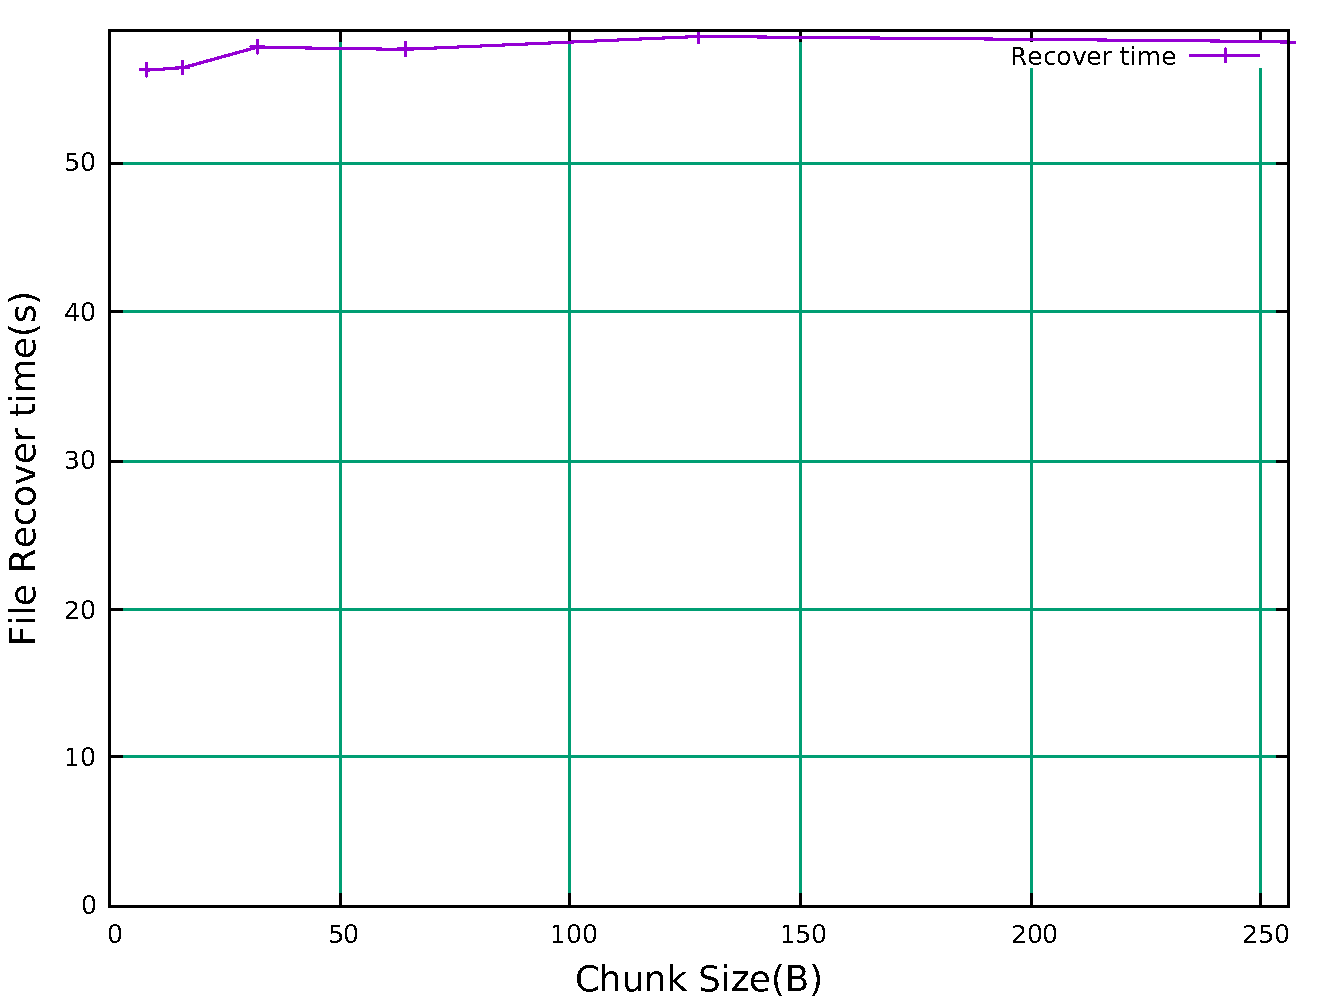
\includegraphics[width=\linewidth]{figures/RAIDRecoverTimeChuckSize5Mb.pdf}
\centering
\caption{Disk Recover time in seconds for varying Chunk sizes under a fixed file size of 5MB}
\label{fig:S3R6RcvCHK5MB}
\end{figure}

\section{LIMITATIONS AND LESSONS}
\label{sec:lessons}

We briefly state the lessons learned here and make an effort to draw deeper conclusions based on our experimental results.
Our experimental draw few conclusions about our design.
The discussion is of two fold.
We discuss advantages of this approach and disadvantages of this approach followed up by best suited applications.

Since our design is based on object storage, the network speed effects the performance of the system.
As you can see from the results, the file size effects the save and recover times for files and disks respectively as each operation requires network connectivity.

As the same time, this concept brings advantages.
Object storage is managed.
Meaning, it is unlikely a user needs to worry about validating the health of storage disks and maintenance. 
Moreover, object storage is elastic.
This entails that a user is free to inflate and shrink the size of RAID6 storage as necessary.
Such advantages cater to a specific need of storage.
More specifically, should there be a need to archive data at very high reliability the proposed approach in this solution is a strong candidate.
Under geographically sparse locations spread across the world, each storage disk maintained under a different vendors, this approach will offer very high reliability.

\section*{Acknowledgments}
The authors would like to thank Prof. Datta for the provided opportunity which aided in exploring a number of technologies related to distributed storage systems.

\balance
\bibliographystyle{ACM-Reference-Format}
\bibliography{reference}

\end{document}